\chapter{Fourier Analysis and Sampling}
\label{chapter:FourierAnalysisSampling}

\emph{Fourier analysis} refers to a collection of tools that can be applied to express a function in terms of sinusoidal components, called basis elements, of different frequencies.
The result of the decomposition is the amplitude and the phase to be imparted to each basis element in the reconstruction.
This decomposition is termed the \emph{frequency domain representation} of the original function.

Fourier analysis is extremely useful in engineering, with a myriad of applications.
Part of its appeal lies in the fact that basis elements are eigenfunctions of linear time-invariant systems.
This properties is instrumental in solving many challenging problems, and makes Fourier analysis a powerful tool for the design of communication systems.


\section{The Fourier Transform}

The Fourier transform discussed below applies to continuous signals.
We assume that the reader is familiar with Fourier analysis, and only review details that are pertinent to our treatment of communication systems.
This is not intended to be a comprehensive treatment of harmonic analysis.

Suppose that $x(t)$ is a continuous signal that is square integrable,
\begin{equation} \label{equation:L2Condition}
\| x(t) \|^2 = \int_t | x(t) |^2 dt < \infty .
\end{equation}
Then, we can express $x(t)$ using its frequency domain representation.
The Fourier transform of $x(t)$, which we denote by $\mathbb{X}(f)$ or $\mathcal{F} [x(t)]$, is defined by
\begin{equation} \label{equation:FourierTransform}
\mathbb{X}(f) = \mathcal{F} [x(t)]
= \int_t x(t) e^{-j 2 \pi f t} dt .
\end{equation}
The original function can then be expressed in terms of its decomposition,
\begin{equation} \label{equation:InverseFourierTransform}
x(t) = \int_f \mathbb{X}(f) e^{j 2 \pi f t} df .
\end{equation}
We sometimes represent the inverse Fourier transform of $\mathbb{X}(f)$ by $\mathcal{F}^{-1} [\mathbb{X}(f)]$.
It is interesting to note the duality between the Fourier transform and its inverse.

\begin{example}[Rectangular Pulse]
The rectangular pulse $\Pi (t)$ defined by
\begin{equation*}
\Pi (t) = \begin{cases} 1, & |t| < 0.5 \\
0, & \text{otherwise} \end{cases}
\end{equation*}
can be used to filter various signals.
Note that $\| \Pi (t) \|^2 = 1 < \infty$.
Its Fourier transform can be computed as follows,
\begin{equation*}
\begin{split}
\mathcal{F} \left[ \Pi(t) \right]
&= \int_t \Pi (t) e^{- j 2 \pi f t} dt
= \int_{-1/2}^{1/2} e^{- j 2 \pi f t} dt \\
&= \frac{1}{\pi f} \left( \frac{e^{j \pi f} - e^{- j \pi f}}{2j} \right)
= \frac{ \sin \pi f }{\pi f} = \mathrm{sinc}(f) .
\end{split}
\end{equation*}
\end{example}

When condition~\eqref{equation:L2Condition} is not satisfied, it may be hazardous to use Fourier analysis and frequency domain representations.
Strictly speaking, the Fourier transform of a function may not exist if it behaves wildly.
Casually talking about the Fourier transform of arbitrary signals should be avoided.
Having said that, there will be instances where we discuss the Fourier transforms of functions that do not fulfill \eqref{equation:L2Condition};
one such example appears below.
We adopt this somewhat cavalier attitude because experience allows us to avoid pitfalls, and Fourier relaxation leads to great engineering insight.
The downside of this approach is that the reader is left with the burden of deciding whether a signal has a proper spectral representation, or if the definition of the Fourier transform is applied loosely.

Starting with signal $x(t)$, we can write
\begin{equation} \label{equation:NestedFourierRepresentation}
\begin{split}
x(t) &= \int_f \mathbb{X}(f) e^{j 2 \pi f t} df \\
&= \int_f \left[ \int_\tau x(\tau) e^{-j 2 \pi f \tau} d\tau \right] e^{j 2 \pi f t} df \\
&= \int_\tau \left[ \int_f e^{j 2 \pi f (t - \tau)} df \right] x(\tau) d\tau ,
\end{split}
\end{equation}
where the second equality follows from \eqref{equation:FourierTransform} and the third equality is obtain by changing the order of integration.
Recall that we can use a $\delta$-function representation to write
\begin{equation*}
x(t) = \int_{\tau} \delta (t - \tau) x(\tau) d\tau .
\end{equation*}
Looking at \eqref{equation:NestedFourierRepresentation}, we gather that
\begin{equation*}
\delta (t) = \int_f e^{j 2 \pi f t} df
\end{equation*}
and hence the (cavalier) Fourier transform of the $\delta$-function is $\mathcal{F} [ \delta(t) ] = 1$.


\subsection{Periodic Signals}

We can develop a (cavalier) Fourier transform representation for periodic signals as well, thereby providing a unified treatment of periodic and aperiodic signals. 
Indeed, we can construct the Fourier transform of a periodic signal directly from its Fourier series representation.
Let $x(t)$ be a signal with Fourier transform $\mathbb{X}(f) = \delta (f - f_0)$.
To recover the signal $x(t)$, we can apply the inverse Fourier transform
\begin{equation*}
x(t) = \mathcal{F}^{-1} [ \delta (f - f_0) ]
=\int_f \delta (f - f_0) e^{j 2 \pi ft} df
= e^{j 2 \pi f_0 t}.
\end{equation*}
More generally, if $\mathbb{X}(f)$ is a linear combination of impulses equally spaced in frequency
\begin{equation} \label{equation:PeriodicFrequency}
\mathbb{X}(f) = \sum_{n = -\infty}^{\infty} c_n \delta (f - n f_0) ,
\end{equation}
then its inverse Fourier transform becomes
\begin{equation} \label{equation:PeriodicTime}
x(t) = \sum_{n = -\infty}^{\infty} c_n e^{j 2 \pi n f_0 t} .
\end{equation}
Note that \eqref{equation:PeriodicTime} corresponds to the Fourier series representation of a periodic signal.
Thus, the Fourier transform of a periodic signal with Fourier series coefficients $\{ c_n \}$ can be interpreted as a train of impulses in the frequency domain.

A signal that will be useful in our analysis of sampling is the impulse train
\begin{equation*}
x(t) = \sum_{n = -\infty}^{\infty} \delta(t - nT_0) .
\end{equation*}
This is a special case of a periodic function, with period $T_0$.
We can therefore apply a methodology similar to the one derived above to compute its Fourier transform.
The Fourier series coefficients for the impulse train are given by
\begin{equation*}
c_n = \frac{1}{T_0} \int_{-T_0/2}^{T_0/2} x(t) e^{- j 2 \pi \frac{n}{T_0} t} dt
= \frac{1}{T_0} .
\end{equation*}
Using \eqref{equation:PeriodicFrequency}, we get
\begin{equation} \label{equation:ImpulseTrainFrequency}
\mathbb{X}(f) = \frac{1}{T_0} \sum_{n = -\infty}^{\infty} \delta \left( f - \frac{n}{T_0} \right) .
\end{equation}
An impulse train in the time domain can be regarded as an impulse train in the frequency domain.
A second representation for $x(t)$ is given by \eqref{equation:PeriodicTime},
\begin{equation} \label{equation:ImpulseTrainTime}
x(t) = \sum_{n = -\infty}^{\infty} \delta(t - nT_0)
= \frac{1}{T_0} \sum_{n = -\infty}^{\infty} e^{j 2 \pi \frac{n}{T_0} t} .
\end{equation}
Which representation to use depends on the problem at hand.


\subsection{Spectral Density}
\label{subsection:SpectralDensity}

The energy content of a deterministic signal $x(t)$ is given by \eqref{equation:L2Condition}.
If the energy content of $x(t)$ is finite, i.e.\ $\| x(t) \|^2 < \infty$, then we can define its \emph{time autocorrelation function} by
\begin{equation*}
R_x(\tau) = \int_t x(t)x^*(t - \tau) dt .
\end{equation*}
Using this notation, we can write the energy content of $x(t)$ as $R_x(0)$.

\begin{definition}
The \emph{energy spectral density} of $x(t)$, denoted by $\mathcal{G}_x (f)$, is the Fourier transform of its time autocorrelation function,
\begin{equation*}
\mathcal{G}_x(f) = \mathcal{F} [ R_x (\tau) ] = | \mathbb{X}(f) |^2.
\end{equation*}
\end{definition}

Intuitively, the energy spectral density captures the frequency content of a signal and helps identify how its energy is distributed across frequencies.
The \emph{spectral bandwidth} of deterministic signal $x(t)$ is the smallest value of $W$ such that $\mathcal{G}_x(f) = 0$ for all $|f| > W$.
Note that if $x(t)$ has bandwidth $W$, then the Fourier transform of $x(t)$ is identically zero for all $|f| > W$.


\subsection{Linear Time-Invariant Filters}
\label{subsection:LinearTimeInvariantFilters}

The importance of the Fourier transform comes, partly, from its ability to characterize the effects of linear time-invariant filters on deterministic signals.
Suppose that the input to the filter is $x(t)$, then the output of the filter is given by
\begin{equation*}
y(t) = x(t) \star h(t),
\end{equation*}
where $h(t)$ is the impulse response of the linear filter and $\star$ denotes the convolution operator.
If we use $\mathbb{H}(f)$ to represent the Fourier transform of impulse response $h(t)$, then the output signal in the frequency domain becomes
\begin{equation*}
\mathbb{Y}(f) = \mathbb{X}(f) \mathbb{H}(f) .
\end{equation*}
That is, convolution in the time domain becomes multiplication in the frequency domain, a much simpler operation.
The output signal can then be recovered by taking the inverse Fourier transform of $\mathbb{Y}(f)$,
\begin{equation*}
y(t) = \mathcal{F}^{-1} [ \mathbb{Y}(f) ] = \mathcal{F}^{-1} [ \mathbb{X}(f) \mathbb{H}(f) ] .
\end{equation*}
\section{Sampling Deterministic Signals}

The sampling theorem is one of the most important results in communications.
Many digital communication systems rely on the validity of this theorem and on the design insights it provides for proper operation.
The basic idea behind the sampling theorem can be summarized in a few words.
If the continuous signal $x(t)$ is bandlimited to $W$, then this signal can be reconstructed from its samples so long as they are taken at periodic intervals of $T_0 \leq \frac{1}{2W}$.
A formal version of the sampling theorem appears below.

\begin{theorem}[Sampling Theorem] \label{theorem:SamplingTheorem}
Suppose that $x(t)$ is a bandlimited signal with bandwidth $W$.
If $x(t)$ is sampled at times $t = 0, \pm T_0, \pm 2T_0, \ldots$ where $T_0 \leq \frac{1}{2W}$, then it is possible to reconstruct the original signal $x(t)$ perfectly from its sampled points $\{ x(nT_0) : n = 0, \pm 1, \pm 2, \ldots \}$.
Indeed, if $T_0 \leq \frac{1}{2W}$ then
\begin{equation*}
x(t) = \sum_{n = -\infty}^{\infty}
x(nT_0) \mathrm{sinc} \left( \left( \frac{t}{T_0}-n \right) \right) .
\end{equation*}
\end{theorem}
\begin{proof}
Let $x_{s}(t)$ denote the result of sampling $x(t)$ by impulses at times $\{ nT_0 \}$,
\begin{equation*}
x_s(t) = x(t) \sum_{n=-\infty}^{\infty} \delta(t-nT_0)
= \sum_{n=-\infty}^{\infty} x(nT_0) \delta(t-nT_0).
\end{equation*}
Looking at the sampled signal in the frequency domain, we get
\begin{equation*}
\begin{split}
\mathbb{X}_s(f) &= \mathbb{X}(f) \star \mathcal{F} \left[ \sum_{n=-\infty}^{\infty} \delta(t-nT_0) \right] \\
&= \mathbb{X}(f) \star \frac{1}{T_0} \sum_{n=-\infty}^{\infty} \delta \left( f-\frac{n}{T_0} \right) \\
&= \frac{1}{T_0} \sum_{n=-\infty}^{\infty} \mathbb{X} \left( f - \frac{n}{T_0} \right) ,
\end{split}
\end{equation*}
where we have used \eqref{equation:ImpulseTrainFrequency} to express the Fourier transform of an impulse train.

Passing the sampled signal through an ideal lowpass filter defined by
\begin{equation*}
\mathbb{H}(f) = T_0 \Pi \left( \frac{f}{2W} \right)
= \begin{cases} T_0, & |f| < W \\
0, & |f| > W \end{cases}
\end{equation*}
we obtain the output
\begin{equation*}
\mathbb{X}_s(f) \mathbb{H}(f)
= \frac{1}{T_0} \left[ \sum_{n=-\infty}^{\infty} \mathbb{X} \left( f - \frac{n}{T_0} \right) \right]
T_0 \Pi \left( \frac{f}{2W} \right)
= \mathbb{X}(f) .
\end{equation*}
The output of the ideal lowpass filter $\mathbb{H}(f)$ is the original signal $x(t)$, and perfect reconstruction is achieved.
The sampling rate corresponding to $T_0 = \frac{1}{2W}$ is the minimum sampling rate at which no aliasing occurs.
It is called the \emph{Nyquist rate}.
\end{proof}

A succession of power spectral densities can be found on Figure~\ref{figure:Sampling}.
\begin{figure}[htbp]
\begin{center}
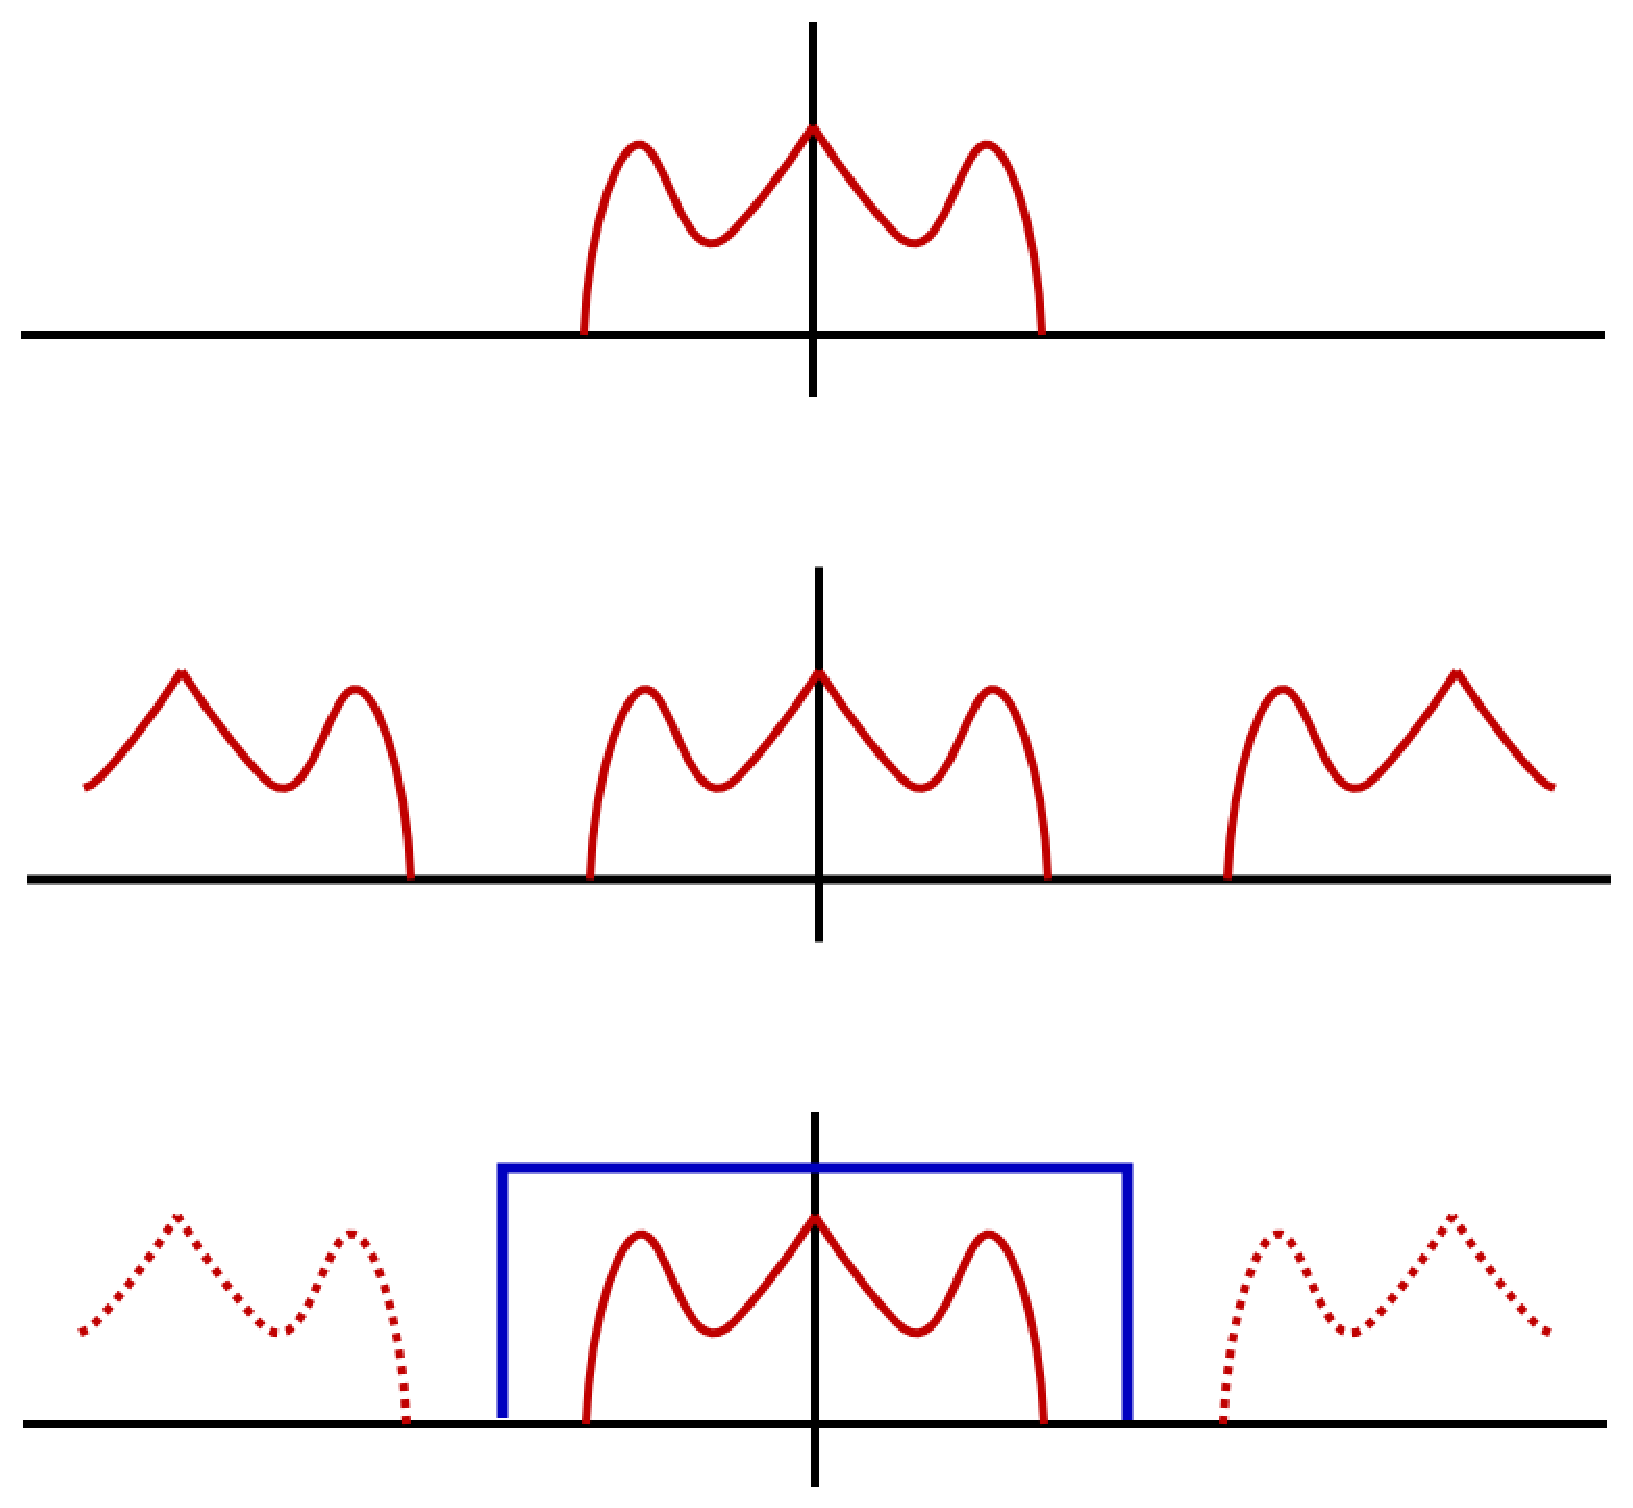
\epsfig{file=Figures/sampling,width=8cm}
\caption{The sampling and reconstruction of a bandlimited signal.}
\label{figure:Sampling}
\end{center}
\end{figure}
The top component shows the power spectral density of the original signal.
The density of the sampled signal appears below.
Finally, the reconstruction operation where a lowpass filter is employed to recovered the original signal is illustrated at the bottom of the figure.
In contrast, Figure~\ref{figure:Aliasing} exhibits a case where the sampling frequency is too low.
\begin{figure}[htbp]
\begin{center}
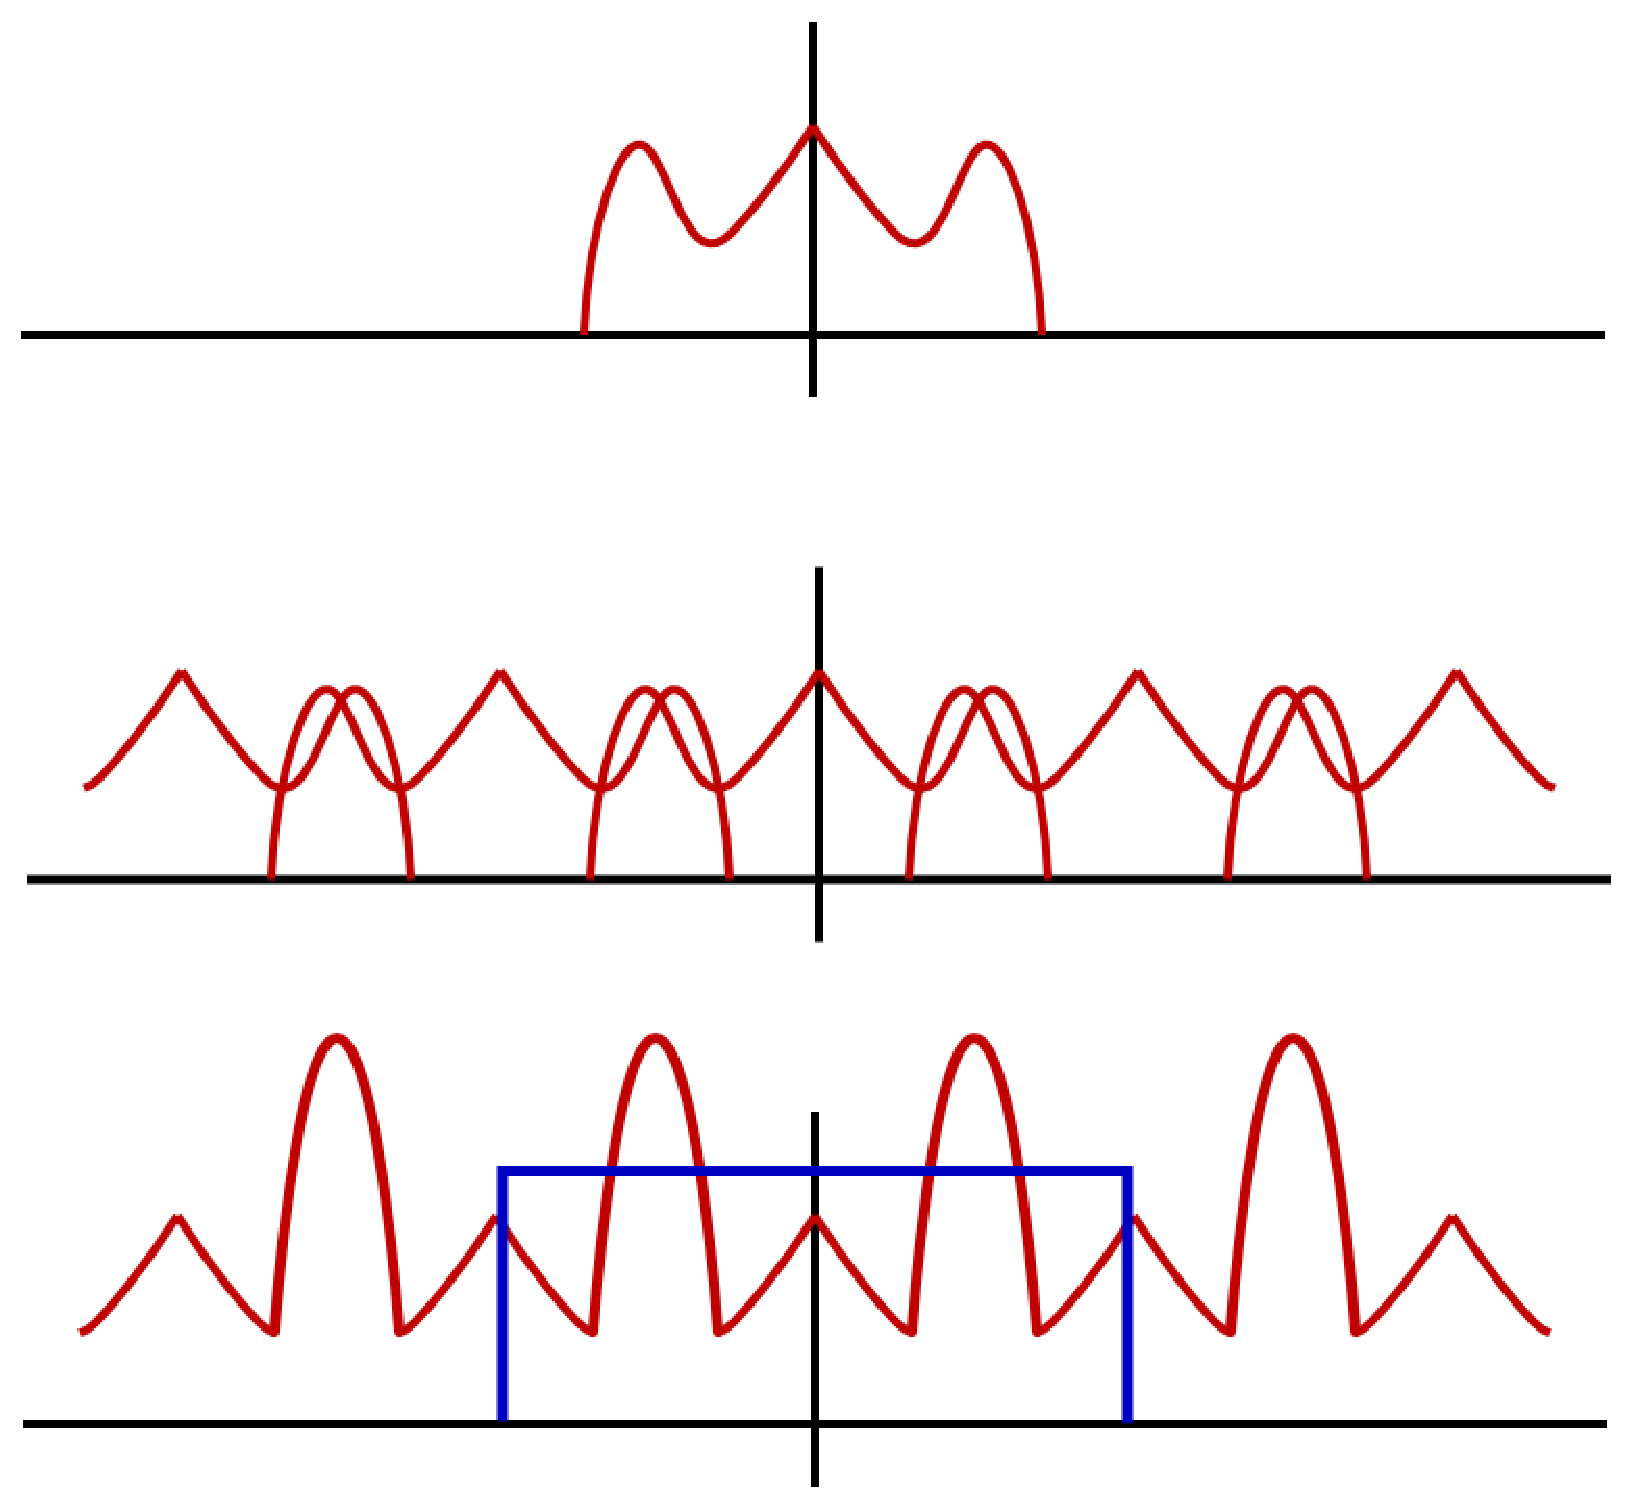
\epsfig{file=Figures/aliasing,width=8cm}
\caption{A low sampling frequency leads to aliasing, thereby preventing reconstruction of the original signal.}
\label{figure:Aliasing}
\end{center}
\end{figure}
Aliasing in the frequency domain prevents the original signal from being retrieved.

The illusion of a moving image in video is achieved by displaying a rapid succession of still pictures over time.
Films are typically shot at a rate of twenty-four frames per second, whereas the minimum frame rate required to create the appearance of a moving image is about fifteen frames per second.
The human eye acts as a lowpass filter and transforms the succession of images into a live video.
High-speed cameras are used to record slow-motion playback movies.
As a consequence, they must run at much higher frame rates than normal cameras.


\section{Stochastic Signals}
\label{section:StocahsticSignalsFAS}

A \emph{stochastic process} (or \emph{random process}) is an extension of the concept of \emph{random variable} to the situation where the future values of a signal are not known beforehand.
Mathematically, a stochastic process can be viewed in two different ways.
First, the process can be thought of as an instantiation of a random experiment where the outcome is selected from a collection of time functions.
Alternatively, a stochastic process can be viewed as a collection of random variables indexed by time.
If the index set corresponds to the real numbers, then the process is a \emph{continuous-time random process}.
Whereas if the index set is discrete, then the random process is a \emph{discrete-time random process}.
The viewpoint where a stochastic process is regarded as a collection of random variables tend to prevail in the study of digital communications.
\begin{figure}[htbp]
\begin{center}
\begin{psfrags}
\psfrag{A}[c]{Amplitude}
\psfrag{t}[c]{Time}
\psfrag{t0}[c]{$t_0$}
\psfrag{t1}[c]{$t_1$}
\epsfig{file=Figures/process,width=7cm}
\end{psfrags}
\caption{Two distinct views of a random process.}
\label{figure:RandomProcess}
\end{center}
\end{figure}

Random processes are frequently employed in the design of communication systems.
For example, they can be used to model the data originating from a source, channel variations, noise and interference.
Their importance will become evident as we progress through these notes.
In general, it is difficult to provide a complete mathematical description for a random process.
For now, we restrict our attention to \emph{stationary} and \emph{ergodic} random processes.

\begin{definition}[Stationarity]
A random process $x(t)$ is wide-sense stationary if its \emph{mean}
\begin{equation*}
m_x(t) = \mathrm{E} [x(t)]
\end{equation*}
is independent of time, and its \emph{autocorrelation function} defined by
\begin{equation*}
R_x(t_1, t_2) = \mathrm{E} [x(t_1) x^*(t_2)]
\end{equation*}
only depends on the difference between $t_1$ and $t_2$.
With a slight abuse of notation, we can denote the mean and autocorrelation of a stationary process by $m_x$ and $R_x(\tau)$ where $\tau = t_1 - t_2$.
\end{definition}

\begin{definition}[Ergodicity]
The \emph{ergodic theorems} assert that, under certain conditions, the time average of a function along all the possible trajectories of a random process exists and is equal to its ensemble average,
\begin{equation*}
\lim_{T \rightarrow \infty} \frac{1}{T} \int_{- \frac{T}{2}}^{\frac{T}{2}} g(x(t)) dt
= \mathrm{E}[g(x(t))] .
\end{equation*}
When a stochastic process fulfills these conditions, it is called \emph{ergodic}.
\end{definition}

\begin{figure}[htbp]
\begin{center}
\begin{psfrags}
\psfrag{A}[c]{Amplitude}
\psfrag{t}[c]{Time}
\psfrag{t0}[c]{$t_0$}
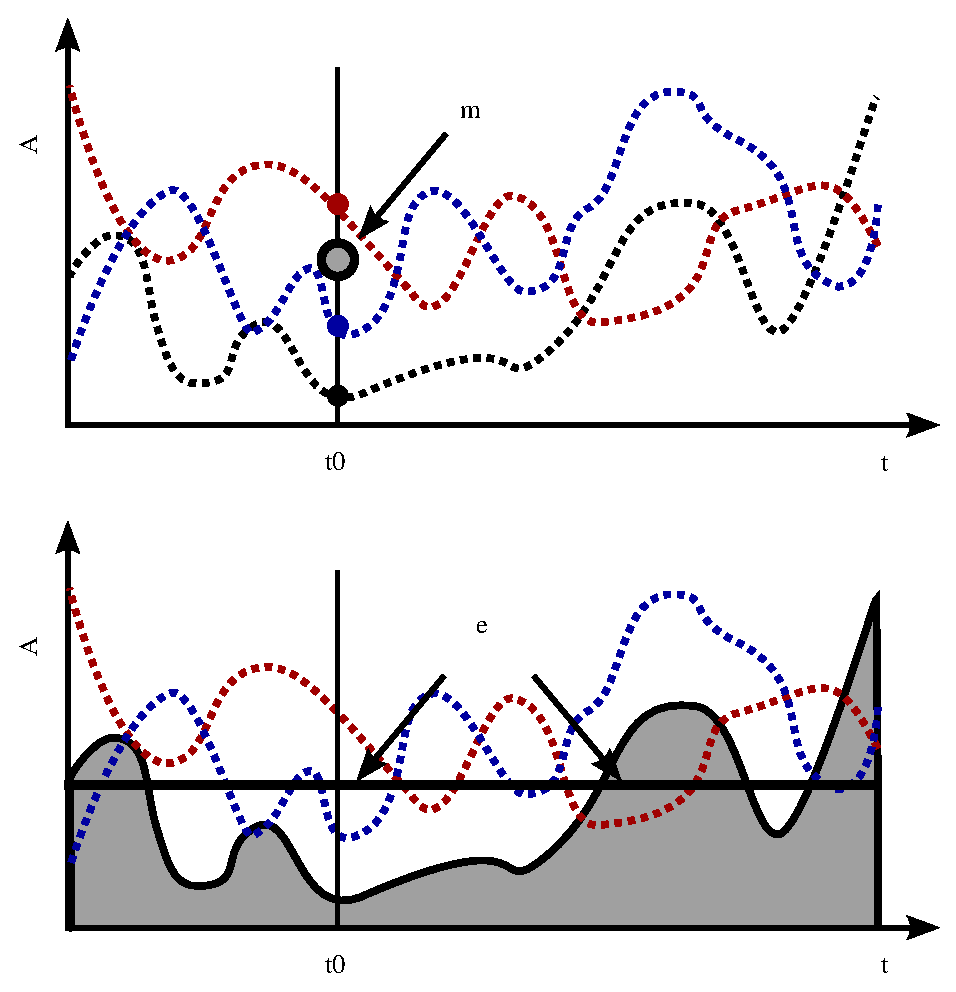
\epsfig{file=Figures/ergodic,width=8cm}
\end{psfrags}
\caption{For ergodic processes, the time average of a function along a trajectory is equal to the ensemble average.}
\label{figure:ErgodicProcess}
\end{center}
\end{figure}

One of the important characteristics of an ergodic process is that it suffices to look at one realization of the process to infer many of its statistical attributes.
Ergodicity is a very strong property, and it is hard to test and validate.
Rather, it is frequently taken as a premise in the design of communication systems.
For instance, most information sources are assumed to be stationary and ergodic.
Such a postulate appears reasonable, especially given the many successful communication systems implemented to date.


\subsection{Power Spectral Density}

The \emph{power spectral density} of a stochastic signal is an extension to the spectral density discussed in Section~\ref{subsection:SpectralDensity}.
The definition of the power spectral density is somewhat more intricate due to the more complex nature of random signals.
In particular, it must account for uncertainty in the process.

Let $x(t)$ be a wide-sense stationary and ergodic random process.
The Fourier transform of a specific realization of $x(t)$ may not exist, as it need not fulfill condition \eqref{equation:L2Condition}.
However, a truncated version of $x(t)$ always possesses a Fourier transform.
Let $x_T(t)$ be the truncated version of $x(t)$ given by
\begin{equation*}
x_T(t) = \begin{cases} x(t), & |t| < \frac{T}{2} \\
0, & \text{otherwise} . \end{cases}
\end{equation*}
The power spectral density of $x(t)$ represents the amount of power per hertz of bandwidth present in the signal at various frequencies, and it is defined by
\begin{equation*}
\mathcal{S}_x(f) = \lim_{T \rightarrow \infty} \frac{1}{T} \mathrm{E} \left[ |\mathbb{X}_T(f)|^2 \right] .
\end{equation*}
Note how the truncated signal is used to overcome the difficulty of dealing with infinite-energy signals.
This is a common trick.
As we will soon see, the power spectral density plays an instrumental role in the sampling theorem for random signals.
First, we provide a means to compute $\mathcal{S}_x(f)$ from its statistical attributes.

\begin{theorem}[Wiener-Khinchin]
The power spectral density $\mathcal{S}_x (f)$ of a wide-sense stationary random process $x(t)$ is equal to the Fourier transform of its autocorrelation function, $\mathcal{S}_x (f) = \mathcal{F} [R_x (\tau)]$.
\end{theorem}
\begin{proof}
For a wide-sense stationary process, we have
\begin{equation*}
\begin{split}
\mathcal{S}_x(f) &= \lim_{T \rightarrow \infty} \frac{1}{T} \mathrm{E} \left[ |\mathbb{X}_T(f)|^2 \right]
= \lim_{T \rightarrow \infty} \frac{1}{T} \mathrm{E} \left[ \mathbb{X}_T(f) \mathbb{X}_T^*(f) \right] \\
&= \lim_{T \rightarrow \infty} \frac{1}{T} \mathrm{E} \left[
\int_{-\frac{T}{2}}^{\frac{T}{2}} x(t_1) e^{-j2 \pi f t_1} dt_1
\int_{-\frac{T}{2}}^{\frac{T}{2}} x^*(t_2) e^{j2 \pi f t_2} dt_2 \right] \\
&= \lim_{T \rightarrow \infty} \frac{1}{T}
\int_{-\frac{T}{2}}^{\frac{T}{2}} \int_{-\frac{T}{2}}^{\frac{T}{2}}
\mathrm{E} \left[ x(t_1) x^*(t_2) \right]
e^{-j2 \pi f (t_1-t_2)} dt_1 dt_2 \\
&= \int_{\tau} R_x (\tau) e^{-j2 \pi f\tau} d\tau
= \mathcal{F} [ R_x (\tau) ] .
\end{split}
\end{equation*}
The fourth equality is obtained by interchanging the expectation and the integrals, while the sixth equality follows from a change of variables and the fact that $x(t)$ is wide-sense stationary.
To guarantee that the former operation is legitimate, $\tau R_x(\tau)$ must remain finite for all $\tau$.
\end{proof}


\subsection{Filtering Stochastic Processes}

We discussed in Section~\ref{subsection:LinearTimeInvariantFilters} how the Fourier transform can simplify the analysis of the effects of linear time-invariant filters on deterministic signals.
In this section, we consider the operation of such filters in the context of random processes.

\begin{theorem}
If a wide-sense stationary process $x(t)$ with mean $m_x$ and autocorrelation function $R_x(\tau)$ is passed through a linear time-invariant filter with impulse response $h(t)$, then output process has mean
\begin{equation*}
m_y = m_x \int_{-\infty}^{\infty} h(t) dt
\end{equation*}
and its autocorrelation is equal to
\begin{equation*}
R_y (\tau) = R_x(\tau) \star h(\tau) \star h^*(-\tau) .
\end{equation*}
\end{theorem}
\begin{proof}
The output process at time~$t$ is given by $y(t) = \int_{-\infty}^{\infty} x(t - \xi) h(\xi) d\xi$.
We can therefore obtain the expectation of $y(t)$ as follows,
\begin{equation*}
\begin{split}
m_y (t) &= \mathrm{E} \left[ \int_{-\infty}^{\infty} x(t - \xi) h(\xi) d\xi \right] \\
&= \int_{-\infty}^{\infty} \mathrm{E} \left[ x(t - \xi) \right] h(\xi) d\xi \\
&= m_x \int_{-\infty}^{\infty} h(\xi) d\xi.
\end{split}
\end{equation*}
We emphasize that $m_y$ is independent of time.

To derive the autocorrelation function for $y(t)$, we first compute the cross-correlation between $x(t)$ and $y(t)$,
\begin{equation} \label{equation:CrossCorrelationLTI}
\begin{split}
\mathrm{E} [x(t_1) y^*(t_2) ]
&= \mathrm{E} \left[ x(t_1) \int_{-\infty}^{\infty} x^*(\xi) h^*(t_2 - \xi) d\xi \right] \\
&= \int_{-\infty}^{\infty} \mathrm{E} \left[ x(t_1) x^*(\xi) \right] h^*(t_2 - \xi) d\xi \\
&= \int_{-\infty}^{\infty} R_x(t_1 - \xi) h^*(t_2 - \xi) d\xi \\
&= \int_{-\infty}^{\infty} R_x(\tau - \xi) h^*(- \xi) d\xi \\
&= R_x(\tau) \star h^*(-\tau) .
\end{split}
\end{equation}
This clearly shows that the cross-correlation between $x(t)$ and $y(t)$ depends only on $\tau$; we can therefore write it as $R_{xy}(\tau)$.
We are now ready to compute the autocorrelation function for $y(t)$.
\begin{equation} \label{equation:AutoCorrelationLTI}
\begin{split}
\mathrm{E} [y(t_1) y^*(t_2) ]
&= \mathrm{E} \left[ \int_{-\infty}^{\infty} x(\xi) h(t_1 - \xi) d\xi y^*(t_2) \right] \\
&= \int_{-\infty}^{\infty} \mathrm{E} \left[ x(\xi) y^*(t_2) \right] h(t_1 - \xi) d\xi \\
&= \int_{-\infty}^{\infty} R_{xy}(\xi - t_2) h(t_1 - \xi) d\xi \\
&= \int_{-\infty}^{\infty} R_{xy}(\xi) h(\tau - \xi) d\xi \\
&= R_{xy}(\tau) \star h(\tau) .
\end{split}
\end{equation}
Substituting $R_{xy} (\tau)$ by the equivalent expression $R_x(\tau) \star h^*(-\tau)$ from \eqref{equation:CrossCorrelationLTI}, we get the desired result.
We observe that the autocorrelation of the process $y(t)$ only depends on the difference between $t_1$ and $t_2$, and hence $y(t)$ is also wide-sense stationary.
\end{proof}

Obtaining an expression for the autocorrelation function corresponding to the output of a linear time-invariant filter allows us to characterize the power spectral density of the output process.
In terms of the frequency representation, we get $m_y = m_x H(0)$ and
\begin{equation*}
\begin{split}
\mathcal{S}_y (f) &= \mathcal{F} [ R_y (\tau) ] \\
&= \mathcal{F} \left[ R_x (\tau) \star h(\tau) \star h^*(-\tau) \right] \\
&= \mathcal{S}_X(f) |\mathbb{H}(f)|^2 .
\end{split}
\end{equation*}
Not too surprisingly, a linear time-invariant filter can be employed to constrain the bandwidth of a stochastic process.
This is an important result nevertheless, as a linear filter can be used to reduce the bandwidth of a random signal before sampling and to reconstruct a random signal from its samples.


\section{Sampling Bandlimited Processes}

We know from Theorem~\ref{theorem:SamplingTheorem} that a bandlimited signal can be perfectly reconstructed from its samples provided that the sampling rate exceeds twice the bandwidth of the original signal.
At this point, one may wonder whether it is possible to extend the sampling theorem to bandlimited stochastic processes.
This question is answered below.

\begin{theorem} \label{theorem:SamplingRandomSignals}
Suppose that $x(t)$ is a wide-sense stationary bandlimited process with bandwidth $W$ and power spectral density $\mathcal{S}_x (f)$.
Let $\hat{x}(t)$ be the estimate for $x(t)$ built from the sampled values $\{ x(nT_0) : n = 0, \pm 1, \pm 2, \ldots \}$; that is,
\begin{equation*}
\hat{x}(t) = \sum_{n=-\infty}^{\infty} x(nT_0) \mathrm{sinc} (2 W (t - nT_0))
\end{equation*}
where $T_0 = \frac{1}{2W}$ denotes the sampling interval.
Then the mean-squared error between the original random process and its estimate vanishes,
\begin{equation} \label{equation:SamplingMSE}
\| x(t) - \hat{x}(t) \|^2
= \mathrm{E} \left[ \left| x(t) - \sum_{n=-\infty}^{\infty}
x(nT_0) \mathrm{sinc} (2 W (t - nT_0)) \right|^2 \right] = 0 .
\end{equation}
The expectation in \eqref{equation:SamplingMSE} is over all possible realizations of $x(t)$.
\end{theorem}
\begin{proof}
To establish this result, we expand the mean-squared error of \eqref{equation:SamplingMSE},
\begin{equation*}
\begin{split}
&\| x(t) - \hat{x}(t) \|^2
= \mathrm{E} \left[ \left| x(t) - \sum_{n=-\infty}^{\infty} x(nT_0)
\mathrm{sinc}(2 W (t - nT_0)) \right|^2 \right] \\
&= R_x(0) - \sum_{n=-\infty}^{\infty} [ R_x(t-nT_0) + R_x^*(t-nT_0) ]
\mathrm{sinc}(2 W (t - nT_0)) \\
&+ \sum_{n=-\infty}^{\infty} \sum_{m=-\infty}^{\infty} R_x((m-n)T_0)
\mathrm{sinc}(2 W (t - mT_0)) \mathrm{sinc}(2 W (t - nT_0)) .
\end{split}
\end{equation*}
The double summation above can be rewritten as
\begin{equation*}
\begin{split}
&\sum_{n=-\infty}^{\infty} \sum_{p=-\infty}^{\infty} R_x(pT_0)
\mathrm{sinc}(2 W (t - pT_0 - nT_0)) \mathrm{sinc}(2 W (t - nT_0)) \\
&\sum_{n=-\infty}^{\infty} \left( \sum_{p=-\infty}^{\infty} R_x(pT_0)
\mathrm{sinc}(2 W (t - pT_0 - nT_0)) \right) \mathrm{sinc}(2 W (t - nT_0)) \\
&= \sum_{n=-\infty}^{\infty} R_x(t - nT_0) \mathrm{sinc}(2 W (t - nT_0)) ,
\end{split}
\end{equation*}
where the last equality follows from the sampling theorem for deterministic signals (Theorem~\ref{theorem:SamplingTheorem}).
Putting these results together, we get
\begin{equation*}
\| x(t) - \hat{x}(t) \|^2
= R_x(0) - \sum_{n=-\infty}^{\infty} R_x^*(t-nT_0) \mathrm{sinc}(2 W (t - nT_0)) .
\end{equation*}
Applying Theorem~\ref{theorem:SamplingTheorem} one more time and noticing that $R_x(0) = R_x^*(0)$, we obtain $\| x(t) - \hat{x}(t) \|^2 = 0$, as desired.
\end{proof}

Theorem~\ref{theorem:SamplingRandomSignals} is significant in that it asserts that the design insights gained from analyzing deterministic signals hold for random signals as well.


\section{Bandpass Signals and Processes}

One possible application of sampling is to take a continuous-time signal and to transform it into a discrete-time signal.
For instance, this operation gives the information coming out of a source, a format more suitable for digital communications.
This prime application of sampling served as the original motivation for our study of the subject.
A second possible application of sampling is the processing of received waveforms at the output of communication channels.
In digital communications, the data often assumes the form of an analog carrier signal modulated by a digital bit stream.
Mathematically, this situation is captured by the equation
\begin{equation*}
y(t) = x(t) \cos (2 \pi f_0 t) .
\end{equation*}
The signal $y(t)$ is a special form of a \emph{bandpass signal}.
Its Fourier transform $\mathbb{Y}(f)$ is non-zero only for frequencies contained in a small neighborhood of carrier frequency $f_0$.
That is, $\mathbb{Y}(f) = 0$ for all frequencies such that $|f - f_0| \geq W$.
To apply the sampling tools derived above to the information bearing signal $x(t)$, we need to shift the corresponding spectrum to the origin.

The Fourier transform of $y(t)$ is given by
\begin{equation*}
\mathbb{Y}(f) = \frac{1}{2} \mathbb{X}(f+f_0) + \frac{1}{2} \mathbb{X}(f - f_0) .
\end{equation*}
Our strategy is to first eliminate $\frac{1}{2} \mathbb{X}(f + f_0)$ from $\mathbb{Y}(f)$, and then to scale and shift $\frac{1}{2} \mathbb{X}(f + f_0)$ back to the origin.
Define the \emph{step function} $u(t)$ by
\begin{equation*}
u (t) = \begin{cases} 1, & t > 0 \\
0, & t < 0. \end{cases}
\end{equation*}
Taking the Fourier transform of $u(t)$, we get
\begin{equation*}
\begin{split}
{\mathcal{F}} [u (t)]
&= {\mathcal{F}} \left[ \frac{1}{2} + \frac{1}{2} \mathrm{sign}(t) \right] \\
&= \frac{1}{2} \delta (f)
- \frac{1}{2} \int_{-\infty}^0 e^{-j2 \pi ft} dt
+ \frac{1}{2} \int_0^{\infty} e^{-j2 \pi ft} dt \\
&= \frac{1}{2} \delta(f)  + \frac{1}{j2 \pi f}.
\end{split}
\end{equation*}
Using the duality property of the Fourier transform, we get
\begin{equation*}
\mathcal{F}^{-1} [u(f)] = \frac{1}{2} \delta(t) + \frac{j}{2 \pi t} .
\end{equation*}
And, by construction, we obtain $\mathbb{X}(f - f_0) = 2 u(f) \mathbb{Y}(f)$.
We can therefore recover the original lowpass signal $x(t)$ as follows,
\begin{equation*}
x(t)
= \left[ y(t) \star \left( \delta (t) + \frac{j}{\pi t} \right) \right] e^{- j2 \pi f_0 t}
= \left[ y(t) + j \left( y(t) \star \frac{1}{\pi t} \right) \right] e^{- j2 \pi f_0 t} .
\end{equation*}
The second component of this signal,
\begin{equation*}
y(t) \star \frac{1}{\pi t} ,
\end{equation*}
is called the \emph{Hilbert transform} of $y(t)$.
Once $x(t)$ is brought back to baseband, the standard sampling theorem applies and a discrete-time version of the signal can be produced.

% Bandpass processes
